\chapter{Markov Chains, Mixing and Slice Variables}\label{ch:kac}\index{Kac, M.}\index{P\'olya, G.}\index{Ehrenfest urn}\index{Feynman Kac formula}

Chapter~\ref{ch:estimation} estimated the gap from simulated data. This chapter asks what limits the simulation itself: Markov chain Monte Carlo for gauge fields, how fast such chains mix and why, for spin systems, that is tied to the decay of correlations, the cluster and multigrid methods that attack critical slowing down, the topological freezing that they do not remove, and the slice variables that turn a hard conditional into a log concave one. It opens with Mark Kac's discussion of models, because the Feynman Kac formula~\cite{Ka49} and Kac's lemma on return times are the exact tools that reappear later. It then takes in turn Jerrum and Sinclair on randomised approximation and rapid mixing, Sokal on autocorrelation, clusters and zeros, and slice sampling with Besag's Markov random fields.

\section{Kac and the Use of Models}\label{sec:c5kac}

Mark Kac thought hard about what a mathematical model is for, and he often illustrated the point with problems that P\'olya had made famous: the random walk that returns home, the urn that refills itself. This section asks whether that discussion is useful for the mass gap. We think it is, at three levels: as a philosophy that justifies the Migdal Kadanoff caricature, as a set of exact results about recurrence and return times that reappear in renormalization and in Monte Carlo, and through the Feynman Kac formula, which is the bridge between the Euclidean measures of this book and the Hamiltonian whose gap we want.

\subsection{Models as caricatures}

In his 1969 essay \emph{Some Mathematical Models in Science}~\cite{Ka69}, Kac argued that the purpose of a model is not to be a faithful copy of reality but to isolate a mechanism so cleanly that its consequences can be computed, and then to ask which features of reality survive. A good model is a caricature: it exaggerates what matters and discards the rest. His own examples included the Ehrenfest urn, which explains how irreversible behaviour can arise from reversible dynamics, and the Kac ring, a deterministic model of the same paradox.

The Migdal Kadanoff ladder of Sections~\ref{ch:mk} and~\ref{ch:verification} is a caricature in exactly Kac's sense. It discards the true geometry of block spin transformations on $\Z^4$ and keeps two operations, a Bayesian product and a convolution, together with the curvature of the group. What survives is asymptotic freedom with a one loop coefficient within three percent of the truth at scale factor $b=2$ (an agreement specific to $b=2$), confinement at every coupling, and a correlation length that is a first passage time. Kac's view tells us how to use such a model: not as evidence that the real theory has a gap, but as a precise statement of which mechanism would produce one, and therefore of what must be compared to make the argument real. That is how Chapter~\ref{ch:path} is framed. P\'olya's own advice in \emph{How to Solve It}, to solve an auxiliary problem first and to specialise before generalising, is the strategy of Chapter~\ref{ch:twod} and Section~\ref{ch:mk}: solve two dimensions exactly, then a caricature of four.

\subsection{P\'olya's walk and marginal dimensions}\label{sec:c5polya}

P\'olya proved in 1921 that simple random walk on $\Z^d$ returns to its starting point with probability one when $d\le2$ and with probability less than one when $d\ge3$; in three dimensions the return probability is about $0.34$. Kac gave a celebrated exposition of this result and of its connection with Brownian motion. The proof turns on whether the expected number of returns, $\sum_n p_n(0,0)$ with $p_n(0,0)\asymp n^{-d/2}$ for even $n$, diverges.

\begin{figure}[t]
\centering
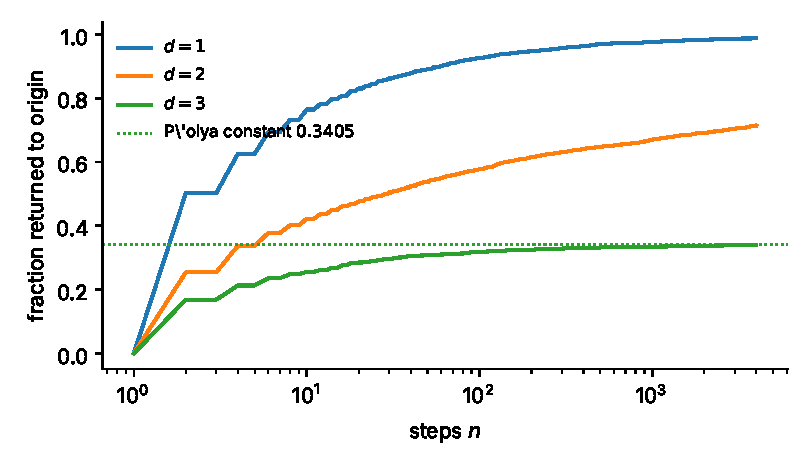
\includegraphics[width=0.85\textwidth]{figures/polya_walk.pdf}
\caption[P\'olya's random walk in one, two and three dimensions]{Fraction of four thousand random walkers that have returned to the origin by step $n$. In one dimension the fraction rises fastest; in two it is certain but logarithmically slow; in three it saturates near P\'olya's constant $0.3405$.}
\label{fig:polya}
\end{figure}

Two dimensions is the marginal case: return is certain, but the expected number of returns grows only like $\log n$, and the walk takes a logarithmically long time to make its point (Figure~\ref{fig:polya}). Four dimensional Yang Mills is the marginal case of the renormalization group in the same sense. The Gaussian ledger of Section~\ref{ch:mk} shows that in flat space the coupling neither grows nor shrinks, and the logarithmic running of asymptotic freedom is the analogue of the logarithmic accumulation of returns. The two cases are not alike in every respect. For the walk, the leading term $p_{2n}(0,0)\sim1/(\pi n)$ already makes the expected number of returns diverge, so recurrence is decided at leading order and the constant $1/\pi$ only sets the rate $\log n$ of that divergence. For Yang Mills the leading order is the neutral Gaussian ledger, and the answer is decided by a correction that is invisible there, the curvature of the group, carried by the Biane Pitman Yor variable.

\subsection{Kac's lemma and the Ehrenfest urn}\label{sec:c5kaclemma}

Kac's lemma says that for a stationary ergodic process, the mean return time to a set $A$ of positive measure, for the process started in $A$, is $1/\pi(A)$. For the Ehrenfest urn with $N$ balls, the mean time to return to a state with $k$ balls in the first urn is $2^N/\binom Nk$, astronomically long for extreme states and short for balanced ones (Figure~\ref{fig:ehrenfest}). This was Kac's resolution of the recurrence paradox: recurrence is guaranteed, but on time scales that make it invisible.

\begin{figure}[t]
\centering
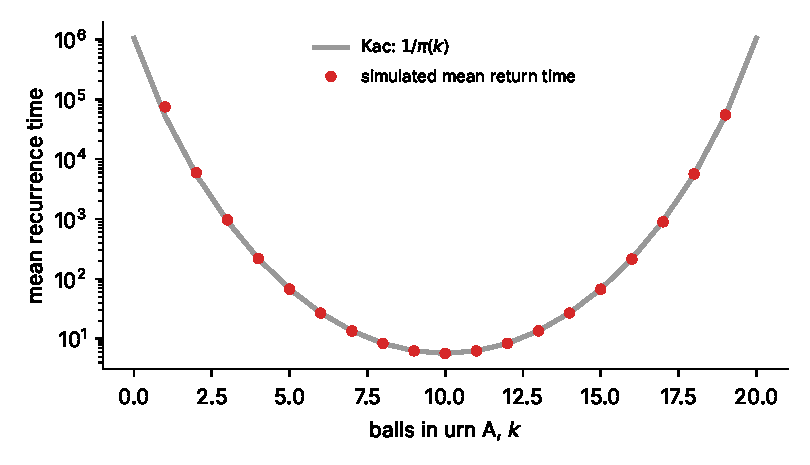
\includegraphics[width=0.85\textwidth]{figures/ehrenfest_kac.pdf}
\caption[Kac's lemma for the Ehrenfest urn]{Mean recurrence time to each state of the Ehrenfest urn with twenty balls, simulated over two million steps, against Kac's formula $1/\pi(k)$.}
\label{fig:ehrenfest}
\end{figure}

The same lemma governs topological freezing in lattice gauge theory. At weak coupling, configurations of nonzero topological charge occupy a small and shrinking fraction of the space accessible to local updates, and the time to tunnel between sectors is at least of the order of the inverse of the probability of the barrier configurations. Kac's lemma converts a statement about rare states into a statement about waiting times, and the split sampling and vertical likelihood methods of Section~\ref{ch:vertical} are, in this light, devices for reweighting the process so that rare states are no longer rare.

\subsection{The Feynman Kac formula}\label{sec:c5fk}

The most important of Kac's contributions for this book is the formula he found in 1949 after hearing Feynman describe path integrals. For a Schr\"odinger operator $H=-\frac12\Delta+V$,
\[
\big(e^{-tH}f\big)(x)=\E_x\Big[\exp\Big(-\int_0^tV(B_s)\,\mathrm ds\Big)f(B_t)\Big],
\]
where $B$ is Brownian motion started at $x$. The semigroup of the Hamiltonian is an expectation over Brownian paths weighted by the Euclidean action. Everything in Chapters~\ref{ch:positivity} and~\ref{ch:routeA} is an infinite dimensional version of this identity: the Euclidean measure on gauge fields is the path measure, the transfer matrix is $e^{-aH}$, and the correlation $C(\tau)=\langle O,e^{-\tau H}O\rangle$ is a Feynman Kac expectation. Reflection positivity is what makes the path measure define a positive semigroup.

The formula also suggests why the mass gap is a large deviation question. The spectral gap of $H$ is the exponential rate at which the Feynman Kac expectation forgets its initial condition. For a single particle in a confining potential this rate is controlled by how rarely Brownian paths wander into regions of high potential, and the Donsker Varadhan theory~\cite{DV75} of large deviations for occupation measures gives a variational formula for the bottom of the spectrum of $H$, though not for the gap above it. In gauge theory the analogue is the rate at which the Euclidean measure decorrelates across time slices.

\subsection{Can one hear the gap?}

Kac's 1966 paper \emph{Can one hear the shape of a drum?}~\cite{Ka66} asked whether the spectrum of the Laplacian determines the domain. His method was the heat trace: $\sum_ne^{-t\lambda_n}$ has a small time expansion whose coefficients are the area and perimeter of the drum and, as Kac conjectured and McKean and Singer~\cite{MS67} proved, its Euler characteristic. The partition functions of two dimensional Yang Mills in Chapter~\ref{ch:twod} are heat traces on the group, and the identity of Section~\ref{ch:riemann} that builds Riemann's kernel from the sphere partition function is a statement about the heat kernel of the three sphere. The mass gap asks for the lowest note of an infinite dimensional drum, and Kac's habit of reading geometry from heat traces is the habit this book has tried to apply.

Kac also left a short commentary~\cite{Ka74}, in P\'olya's collected papers, on how a lemma of P\'olya's about the Riemann $\xi$ function led to the Lee and Yang circle theorem. Chapter~\ref{ch:kacyang} opens with it.

\section{Jerrum, Sinclair and Randomised Polynomial Time}\label{ch:jerrum}\index{Jerrum, M.!and Sinclair, A.}\index{FPRAS}\index{canonical paths}

Is computing a lattice gauge partition function easy or hard? Complexity theory gives a precise answer for the Ising model, and the answer turns on the same structure that drives this book: positivity. This section explains the Jerrum and Sinclair algorithm, what it would mean to have an analogue for gauge theories, and how, for spin systems, rapid mixing of Markov chains is related to decay of correlations, which is not the mass gap.

\subsection{Approximate counting}\label{sec:c5counting}

A fully polynomial randomised approximation scheme (FPRAS) for a quantity $Z$ is a randomised algorithm that, given $\varepsilon$ and $\delta$, returns $\hat Z$ with $(1-\varepsilon)Z\le\hat Z\le(1+\varepsilon)Z$ with probability at least $1-\delta$, in time polynomial in the size of the input, $1/\varepsilon$ and $\log(1/\delta)$. Exact computation of partition functions is typically $\#$P hard. Approximate computation can be easy or hard depending on the model, and the boundary is where much of the interest lies.

\begin{theorem}[Jerrum and Sinclair~\cite{JS93}, 1993]
There is an FPRAS for the partition function of the ferromagnetic Ising model on an arbitrary graph, at any temperature, with a uniform external field.
\end{theorem}

The contrast with the antiferromagnet is a later result, not part of the theorem above: for parameters in the non uniqueness regime of the infinite $r$ regular tree, on the class of graphs of maximum degree $r$, approximate counting for the antiferromagnetic Ising model is NP hard, so no FPRAS exists for that class unless RP equals NP; on a bipartite graph such as $\Z^d$ the zero field antiferromagnet is equivalent to the ferromagnet and is easy (Sly and Sun~\cite{SS12}, and Galanis, \v{S}tefankovi\v{c} and Vigoda~\cite{GSV16}).

The algorithm has two ingredients. The first is a change of representation. The high temperature expansion writes the ferromagnetic Ising partition function as a sum over subgraphs with nonnegative weights, the ``subgraphs world'', and Jerrum and Sinclair built a Markov chain on subgraphs whose stationary law has these weights. The second is a proof of rapid mixing by canonical paths: every pair of states is joined by a path through the chain, and if no transition carries too many paths, the spectral gap of the chain is at most polynomially small. With a rapidly mixing sampler in hand, the partition function follows from a product of ratios along an annealing schedule,
\[
\frac{Z(\beta_K)}{Z(\beta_0)}=\prod_{i=0}^{K-1}\E_{\beta_i}\big[e^{-(\beta_{i+1}-\beta_i)H}\big],
\]
each estimated to small relative error with polynomially many samples. This product estimator is the discrete form of thermodynamic integration and of the power posterior ladder of Section~\ref{ch:vertical}.

\begin{figure}[t]
\centering
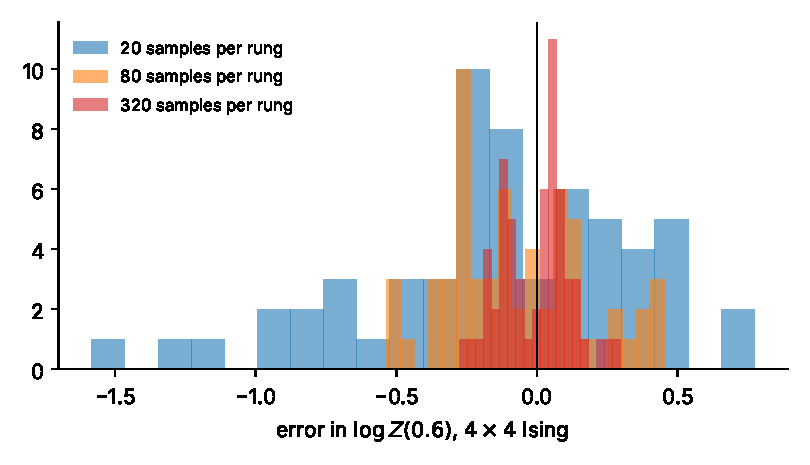
\includegraphics[width=0.85\textwidth]{figures/product_estimator.pdf}
\caption[A product estimator for the $4\times4$ Ising model]{Errors of a twelve rung product estimator for $\log Z(0.6)$ on the $4\times4$ Ising torus, against exact enumeration of all $65{,}536$ states, using Swendsen Wang moves at each rung, sixty repetitions for each sample size. The root mean square error falls from $0.50$ to $0.25$ to $0.12$ as the samples per rung grow from $20$ to $80$ to $320$.}
\label{fig:product}
\end{figure}

\subsection{Why positivity decides complexity}\label{sec:c5positivity}

The ferromagnetic case is easy. In the ferromagnet the high temperature expansion has nonnegative weights, so it defines a probability distribution that a Markov chain can sample. In the antiferromagnet some weights are negative, which is why standard arguments do not apply, but negativity alone does not decide the complexity: hardness holds only in the non uniqueness regime of the tree, as stated above, while in the uniqueness regime and on bipartite graphs in zero field the antiferromagnet is easy (Sly and Sun~\cite{SS12}, Galanis, \v{S}tefankovi\v{c} and Vigoda~\cite{GSV16}). The sign problem of quantum Monte Carlo is a related obstruction, not the same one.

Lattice gauge theory with nonnegative character coefficients, such as the Wilson action, is on the ferromagnetic side as far as the label factors go. The character expansion of Section~\ref{ch:latent} is its high temperature expansion, a sum over decorated surfaces whose weights $c_n$ are nonnegative, which by the Osterwalder Seiler theorem~\cite{OSe} is a sufficient condition for reflection positivity. A ``surfaces world'' Markov chain, the gauge analogue of the subgraphs world, would need the weight of each surface, after the links are integrated out, to be nonnegative; the characters change sign, and Section~\ref{ch:latent} does not claim this. Whether such a chain exists, and whether it mixes rapidly at weak coupling, is not known. The surfaces at weak coupling are large and fluctuating, and canonical path arguments that work for subgraphs have no evident analogue for closed surfaces with representation labels.

\begin{problem}\label{op:mixing1}
Is there an FPRAS for the partition function of SU(2) lattice gauge theory with the Wilson action, on boxes of side $L$, at every coupling, with running time polynomial in $L$?
\end{problem}

\subsection{Rapid mixing and the mass gap}

The question is not only algorithmic. For spin systems, a theorem of Martinelli and Olivieri~\cite{MO94}, building on Dobrushin and Shlosman~\cite{DS85,DS87} and on Stroock and Zegarlinski~\cite{SZ92}, says that for finite range interactions with a finite single spin space on $\Z^d$ the following are equivalent: the Glauber dynamics has a spectral gap, or a logarithmic Sobolev constant, bounded uniformly in the volume and in the boundary conditions; and the Gibbs measure has strong spatial mixing, exponential decay of correlations uniform in the boundary conditions. What the theorem relates is the spectral gap of a Markov chain at a fixed lattice coupling and the rate of decay of correlations of the lattice measure. It does not cover compact continuous spins or gauge fields, and the spectral gap of the chain is not the mass gap of the Hamiltonian, which is the spectral gap of the transfer matrix; nor does it say anything about the continuum limit. Strong spatial mixing uniform in the boundary conditions is also stronger than exponential decay of correlations in one phase: in the low temperature Ising model correlations decay exponentially in each pure phase, while the Glauber gap with free or periodic boundary conditions closes like $e^{-cL^{d-1}}$ on a box of side $L$ (sharp for $d=2$). Section~\ref{ch:dynamic} develops the relation, and Shen, Zhu and Zhu~\cite{SZZ} proved a mass gap for lattice Yang Mills at strong coupling by a stochastic analysis route of a related kind.

So rapid mixing of local Markov chains, the property that Jerrum and Sinclair needed, is connected, for spin systems under the hypotheses above, to exponential decay of correlations at a fixed lattice coupling, a lattice analogue of the property that the Clay problem asks for and not that property. At a critical point, local dynamics slow down polynomially, critical slowing down, and correlations decay polynomially. In a single phase with exponential decay of correlations and no dependence on the boundary, local dynamics mix exponentially fast; at phase coexistence they do not. For Yang Mills the continuum limit is reached as $\beta\to\infty$, where the correlation length in lattice units diverges and local dynamics must slow down. The right question is therefore not whether local dynamics mix rapidly uniformly in $\beta$, which they do not, but whether the relaxation time grows only as a fixed power of the correlation length, $\tau_{\mathrm{rel}}\sim\xi^z$ with $z$ independent of $\beta$ (compare the dynamic exponent in the next section): a statement about the renormalized dynamics along the ladder.

\subsection{Sampling log concave laws}

Our own early work on the complexity of sampling, with Frieze and Kannan~\cite{FKP}, building on Applegate and Kannan~\cite{AK91}, showed that log concave distributions on convex bodies can be sampled in random polynomial time. That result is the continuous analogue of the Jerrum and Sinclair theorem: log concavity plays the role of ferromagnetism, guaranteeing that local moves do not get trapped. Lattice gauge measures are not log concave (on the compact group a geodesically log concave function is constant, Chapter~\ref{ch:path}), and the Bakry \'Emery substitute, a positive lower bound on the Ricci curvature plus the Hessian of $\beta S$, fails at weak coupling because that Hessian is large and indefinite on the scale of the group, which is why the Bakry \'Emery curvature arguments~\cite{BE} of Section~\ref{ch:dynamic} and the stochastic quantization methods of Shen, Zhu and Zhu work only at strong coupling. In the vertical likelihood and P\'olya Gamma constructions, the role of latent variables is to restore log concavity conditionally, and the open question is whether a latent representation of gauge theory can do the same.

\subsection{What the complexity theory gives}

The complexity theory gives three things. The product estimator is the right way to compute partition functions along a renormalization ladder, and its error analysis is directly applicable. The ferromagnetic case, where positivity of the weights holds, is where positivity of the weights gives a Markov chain that can be analysed, which is one reason positivity matters computationally as well as physically. And for spin systems the equivalence between rapid mixing and spatial mixing relates decay of correlations at a fixed lattice coupling to the mixing of Markov chains, a relation whose extension to gauge fields is open and which Chapter~\ref{ch:path} weighs against the other routes.

\section{Sokal: Autocorrelation, Clusters and Zeros}\label{ch:sokal}\index{Sokal, A. D.}\index{autocorrelation time}\index{Edwards, R. G.!and Sokal, A. D.}\index{topological freezing}\index{Lee Yang zeros}

Alan Sokal's work touches almost every computational and structural question in this book. This section collects the parts that matter for the mass gap: the statistics of Markov chain Monte Carlo, cluster representations, multigrid methods, the zeros of partition functions, random walk representations, and the limits of perturbation theory.

\subsection{The statistics of Monte Carlo}\label{sec:c5stats}

Sokal's lecture notes on Monte Carlo methods in statistical mechanics set the standard for how simulation output should be analysed. The central quantity is the integrated autocorrelation time
\[
\tau_{\mathrm{int}}=\tfrac12+\sum_{\ell\ge1}\rho(\ell),
\]
which inflates the variance of a sample mean by a factor $2\tau_{\mathrm{int}}$. Estimating it requires truncating the sum of empirical autocorrelations, because the noise in the partial sum of the empirical autocorrelations grows with the lag. Madras and Sokal's~\cite{MS88} automatic windowing truncates at the first lag $W$ with $W\ge c\,\hat\tau_{\mathrm{int}}(W)$, with $c$ around five or six, balancing bias against variance. Every autocorrelation time in this chapter was estimated that way, with the caveat that where the window cannot close within the run, as at $\beta=6$ below, the estimate is a lower bound.

Sokal also emphasised dynamic critical exponents: near a critical point the autocorrelation time of a local algorithm grows like $\xi^z$ with $z\approx2$, the critical slowing down that made cluster algorithms necessary.

\subsection{Clusters: Edwards and Sokal}\label{sec:c5clusters}

Edwards and Sokal~\cite{ES88} identified the joint distribution of spins and bonds behind the Swendsen and Wang algorithm~\cite{SW87}, and generalised it beyond Potts models. The joint law couples the spin model to the Fortuin Kasteleyn random cluster model~\cite{FK72}, and its conditionals are the two steps of the algorithm: given spins, open bonds between agreeing neighbours independently; given bonds, colour clusters independently. Figure~\ref{fig:sw} shows the payoff on a $24\times24$ Ising torus: near the critical coupling the autocorrelation time of the absolute magnetisation $|M|$ is about twenty sweeps for Metropolis and about four steps for Swendsen and Wang.

\begin{figure}[t]
\centering
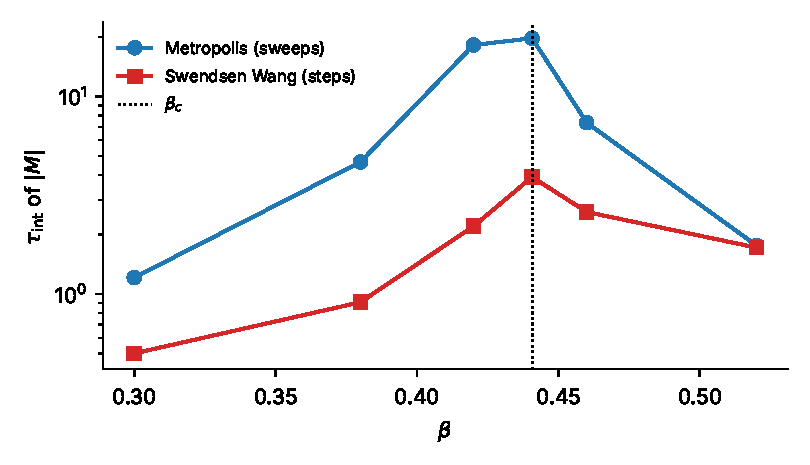
\includegraphics[width=0.85\textwidth]{figures/sw_vs_metropolis.pdf}
\caption[Swendsen Wang against Metropolis near criticality]{Integrated autocorrelation time of $|M|$ on a $24\times24$ Ising torus, estimated by Madras and Sokal windowing, for checkerboard Metropolis and for Swendsen and Wang. The peak at $\beta_c$ is critical slowing down; the cluster algorithm largely removes it.}
\label{fig:sw}
\end{figure}

For this book the Edwards and Sokal construction matters for a second reason. Its joint law is a coupling, and couplings are how monotonicity and decay of correlations are proved for the random cluster model. Chapter~\ref{ch:path} asks for a coupling between a true block spin step and a Migdal Kadanoff step, and the Edwards and Sokal construction is the template.

\subsection{Multigrid Monte Carlo}

Goodman and Sokal~\cite{GS89} introduced multigrid Monte Carlo, which updates the field at a hierarchy of scales by moving coarse grained variables, in direct analogy with multigrid methods for elliptic equations. For Gaussian models it eliminates critical slowing down. For nonlinear models the gain depends on how well the coarse moves respect the effective action at each scale, which is the same question the renormalization group asks. A multigrid sampler for gauge theory whose coarse levels follow the Migdal Kadanoff ladder would be a computational test of the ladder itself.

\subsection{Topological freezing}

The analogue of critical slowing down in lattice gauge theory is topological freezing. In two dimensional U(1) lattice gauge theory the topological charge $Q$, the total winding of the plaquette angles, is an integer, and changing it requires passing through configurations of high action. Figure~\ref{fig:u1} shows Metropolis histories of $Q$ on a $20\times20$ torus: at $\beta=1$ the charge decorrelates in about one sweep, at $\beta=3$ in about thirty six, at $\beta=6$ in more than four hundred, and at $\beta=10$ it did not change once in three thousand sweeps. In four dimensional SU(3) the same phenomenon limits how close to the continuum glueball masses can be measured. Kac's lemma (Section~\ref{sec:c5kaclemma}) gives a lower bound for the growth, and split sampling across sectors from Section~\ref{ch:vertical} is one remedy.

\begin{figure}[t]
\centering
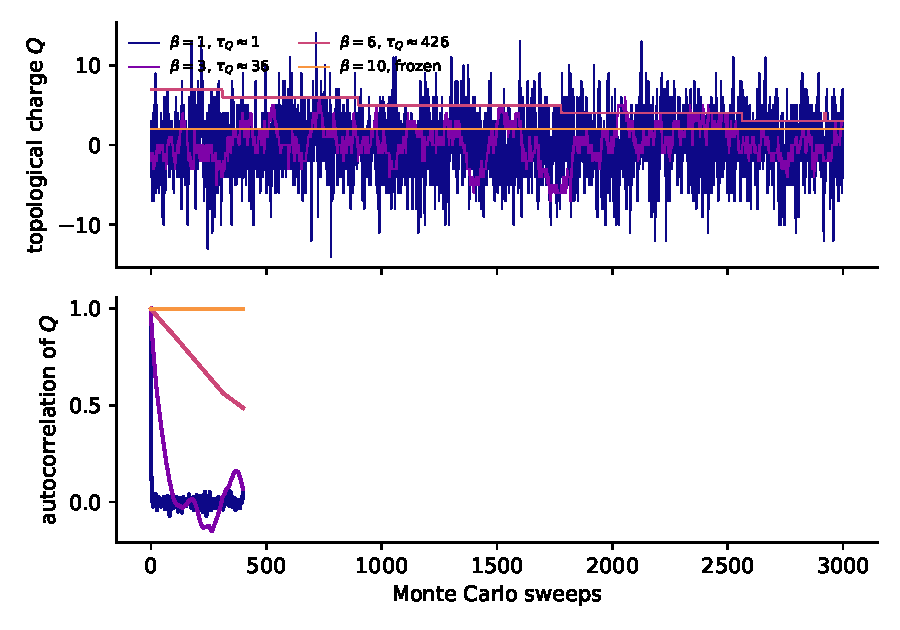
\includegraphics[width=\textwidth]{figures/u1_topology.pdf}
\caption[Topological freezing in two dimensional U(1) lattice gauge theory]{Topological charge histories and autocorrelations for two dimensional U(1) lattice gauge theory on a $20\times20$ torus with Metropolis updates. The integrated autocorrelation time grows from about one sweep at $\beta=1$ to over four hundred at $\beta=6$; at $\beta=10$ the charge is frozen.}
\label{fig:u1}
\end{figure}

\subsection{Zeros of partition functions}\label{sec:c5zeros}

Lee and Yang~\cite{LY52} proved in 1952 that the zeros of the ferromagnetic Ising partition function in the complex fugacity $e^{-2\eta}$ lie on the unit circle. Fisher studied the zeros in the complex temperature, which pinch the real axis at a critical point. Sokal~\cite{So01} extended zero free region results to Potts models and chromatic polynomials, proving that the zeros of the chromatic polynomial of a graph of maximum degree $r$ lie in a disc of radius proportional to $r$, and with Scott~\cite{SS05} connected zero free regions of the hard core gas to the Lov\'asz local lemma.

\begin{figure}[t]
\centering
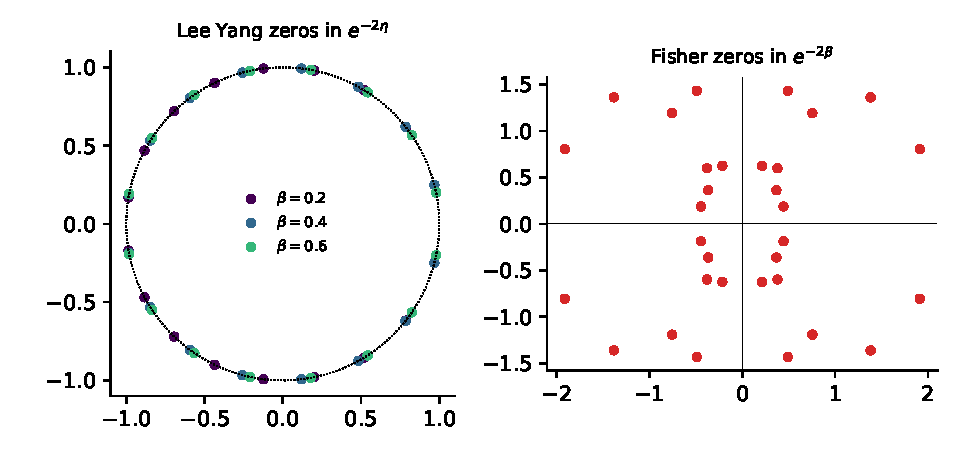
\includegraphics[width=\textwidth]{figures/lee_yang_fisher.pdf}
\caption[Lee Yang and Fisher zeros of the $4\times4$ Ising model]{Left: zeros of the $4\times4$ Ising partition function in $e^{-2\eta}$ at three couplings, all on the unit circle as the Lee Yang theorem requires. Right: zeros in the complex temperature variable $e^{-2\beta}$.}
\label{fig:leeyang}
\end{figure}

Zeros connect three threads of this book. The Lee Yang property is the ferromagnetic random variable condition behind Newman's approach~\cite{Ne76} to the Riemann Hypothesis, which our Riemann programme uses. Zero free regions of a partition function in a complex coupling imply analyticity of the free energy, and analyticity in the coupling across the whole range $0<\beta<\infty$ is exactly the absence of a phase transition that the crossover argument of Chapter~\ref{ch:path} needs. And whether the Fisher zeros of the two dimensional sphere theory can be related, through the identity of Section~\ref{ch:riemann}, to the zeros of $\Xi$ is posed there as an open problem.

\subsection{Random walks, triviality and Borel summability}

Brydges, Fr\"ohlich and Spencer~\cite{BFS82} gave a random walk representation of correlation functions in $\phi^4$ theory, Aizenman and Fr\"ohlich~\cite{Ai82,Fr82} used such representations to prove triviality above four dimensions, and Fern\'andez, Fr\"ohlich and Sokal~\cite{FFS92} gave the systematic account; Aizenman and Duminil Copin~\cite{ADC21} later proved marginal triviality in four. The contrast is instructive: $\phi^4_4$ is marginal and trivial, its coupling running to zero at long distances, while Yang Mills is marginal and asymptotically free, its coupling running to zero at short distances. The two differ by the sign of the one loop term in the beta function. In Section~\ref{ch:mk} that sign is the sign of the curvature of the group, carried by $\E S_{\mathrm{BPY}}>0$.

Sokal's 1980 improvement of Watson's theorem~\cite{So80} gives sharp conditions under which a function is the Borel sum of its asymptotic series. Perturbation theory in Yang Mills is expected to fail those conditions: the series is expected to have renormalon singularities on the positive Borel axis, and a mass gap, if it exists, is a renormalization group invariant mass and so of order $\Lambda=\mu e^{-1/(2b_0g^2)}$, invisible to every order. That is a precise sense in which the gap is nonperturbative, and why the renormalization group must be followed into strong coupling.

\subsection{What Sokal's methods give}

Madras and Sokal windowing is the correct way to quote errors on every Monte Carlo number in this book. Edwards and Sokal is the model for the coupling the comparison step needs. Multigrid is the natural computational test of the ladder. Zero free regions are the analytic form of the no phase transition hypothesis. And the contrast with $\phi^4_4$ isolates the sign that makes Yang Mills different.

\section{Slice Variables, Log Concavity and Besag}\label{ch:slice}\index{slice sampling}\index{Besag, J.}\index{pseudolikelihood}\index{Markov random field}\index{log concavity}\index{Higdon, D.}

Section~\ref{ch:latent} used latent variables as samplers. This section isolates the trick that makes them work, the use of slice variables to turn a hard conditional into a log concave one, in the form given by Polson~\cite{Po96} in 1996 and by Higdon~\cite{Hi98} in 1998. It then applies the trick to the SU(2) link conditional, where positive curvature would turn it into a mixing bound (conditionally on a claim whose proof is only sketched), and asks whether Besag's theory of Markov random fields is useful for the mass gap.

\subsection{The slice variable trick}\label{sec:c5slice}

Let the target be $\pi(x)\propto p(x)\prod_{i=1}^mL_i(x)$ on $\R^d$. Introduce one uniform slice variable $w_i$ for each factor, written $w=(w_1,\dots,w_m)$,
\[
\pi(x,w)\propto p(x)\prod_{i=1}^m\mathrm{I}\{0<w_i<L_i(x)\}.
\]
The $x$ marginal is $\pi$. Given $x$, the $w_i$ are independent uniforms. Given $w$, $x$ has density proportional to $p$ restricted to the set $C(w)=\bigcap_i\{x:L_i(x)>w_i\}$.

\begin{proposition}\label{prop:slicelc}
If $p$ is log concave and every $L_i$ is quasi concave, meaning that its superlevel sets are convex, then for every $w$ the conditional law of $x$ given $w$ is log concave.
\end{proposition}

\begin{proof}
$C(w)$ is an intersection of convex sets, hence convex, and the indicator of a convex set is log concave. A product of log concave functions is log concave.
\end{proof}

The point is that quasi concavity is much weaker than log concavity. A Cauchy likelihood $L(x)=(1+(y-x)^2)^{-1}$ is not log concave, and a posterior built from several of them can be multimodal, but each factor is unimodal, so its superlevel sets are intervals. After slicing, every conditional is a log concave density on a convex set. Frieze, Kannan and Polson~\cite{FKP} showed that such densities can be sampled in time polynomial in the dimension, by a random walk whose conductance is controlled by the isoperimetry of log concave measures. The slice variables thus move the difficulty out of the $x$ conditional and into the slice variables, which are one dimensional, and into the geometry of the sets $C(w)$. This does not make the joint chain rapidly mixing: for a multimodal target the slice levels must still pass through the gaps between modes, and the chain can mix slowly.

Polson's 1996 analysis~\cite{Po96} of the convergence of Markov chain Monte Carlo used the scale mixture version of the same device. Since
\[
\frac{1}{1+z^2}=\int_0^\infty e^{-\lambda(1+z^2)}\,\mathrm d\lambda,
\]
a Cauchy likelihood is a mixture of Gaussian likelihoods over a latent precision. Given the precisions the posterior is Gaussian, hence log concave, but log concavity of one block does not by itself bound the rate of the chain that alternates precisions and location, which is governed by the dependence between the two blocks. This is the same structure as the P\'olya Gamma augmentation of Polson, Scott and Windle~\cite{PSW13} for logistic models, and the same structure as the character expansion of lattice gauge theory, in which a positive latent label renders each conditional tractable (Section~\ref{ch:latent}).

\subsection{Higdon: auxiliary variables and partial decoupling}\label{sec:c5higdon}

Higdon's 1998 paper~\cite{Hi98} organised these ideas for spatial models. For a Potts model with weight $\prod_{\langle ij\rangle}e^{\beta\,\mathrm I\{x_i=x_j\}}$, slicing each bond factor with $w_{ij}\sim\mathrm{Uniform}(0,e^{\beta\mathrm I\{x_i=x_j\}})$ yields the Swendsen and Wang algorithm: a bond whose slice exceeds one forces its endpoints to agree, and the conditional of the spins given the slices is uniform over colourings of the resulting clusters. Partial decoupling slices only a fraction $\delta$ of each factor, $e^{\delta\beta\mathrm I}$, and keeps $e^{(1-\delta)\beta\mathrm I}$ in the conditional, so that clusters are smaller and the remaining interaction keeps the image model faithful. The parameter $\delta$ interpolates between a local heat bath at $\delta=0$ and full Swendsen and Wang at $\delta=1$.

\subsection{Slicing the SU(2) link}

For a link $U$ of two dimensional or four dimensional SU(2) lattice gauge theory, the conditional given its neighbours is
\[
\pi(U\mid\cdot)\propto\exp\Big(\beta\sum_{p\ni U}\tfrac12\operatorname{tr}(UV_p)\Big)\,\mathrm dU,
\]
a product over the plaquettes containing the link, with $V_p$ the staple of plaquette $p$. Identify SU(2) with the unit sphere $S^3$. Each factor is a monotone function of the geodesic distance from $U$ to $V_p^{-1}$, so its superlevel sets are geodesic balls, spherical caps. Slice each plaquette factor separately. Given the slices, $U$ is Haar distributed on the intersection of caps
\[
C(w)=\bigcap_{p\ni U}\big\{U:\tfrac12\operatorname{tr}(UV_p)>c_p\big\}.
\]
The level $c_p$ is related to the slice variable $w_p\in(0,e^{\beta a_p})$ of plaquette $p$, where $a_p=\frac12\operatorname{tr}(UV_p)$, by $c_p=\log w_p/\beta$.

\begin{conjecture}\label{prop:slicecurv}
If every slice level satisfies $c_p>0$, then $C(w)$ is geodesically convex, and the uniform law on $C(w)$, with the reflected Brownian motion on it, satisfies a logarithmic Sobolev inequality with constant $2$, independent of $\beta$ and of the staples.
\end{conjecture}

\begin{proof}[Evidence: sketch of a proof, not a complete proof]
\renewcommand{\qedsymbol}{}
A spherical cap smaller than a hemisphere is geodesically convex in $S^3$, and intersections of geodesically convex sets are geodesically convex. The unit three sphere has Ricci curvature $2$. On a smooth geodesically convex domain of a manifold with $\mathrm{Ric}\ge\kappa>0$, the uniform law with reflecting boundary satisfies the Bakry \'Emery criterion~\cite{BE} with constant $\kappa$, because convexity makes the boundary term in the Bochner formula nonnegative. This is the Bakry \'Emery theorem with a Neumann boundary, for which we have no reference in the bibliography. The set $C(w)$ is an intersection of caps and has corners, so the last step needs an approximation by smooth convex domains, which we do not carry out.
\end{proof}

Figure~\ref{fig:caps} shows the picture one dimension down, on $S^2$: four caps smaller than hemispheres, and their intersection, which is convex.

\begin{figure}[t]
\centering
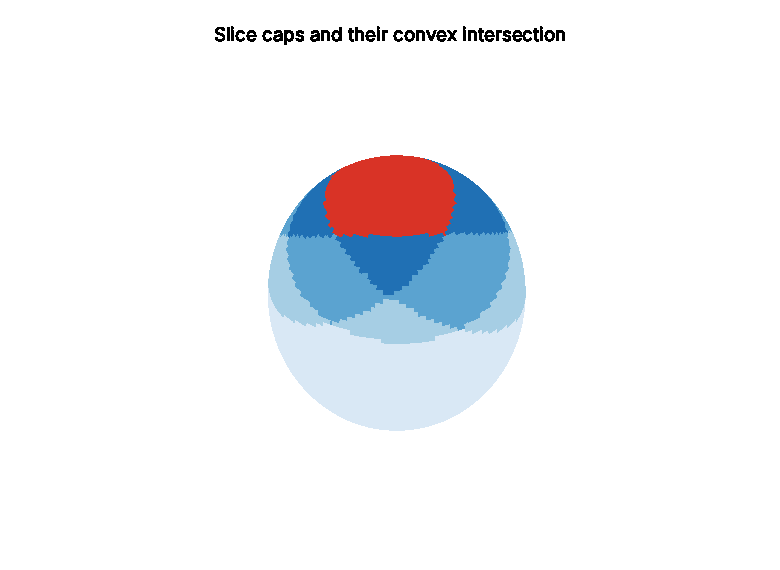
\includegraphics[width=0.7\textwidth]{figures/slice_caps.pdf}
\caption[Slice caps on the sphere]{Four spherical caps on $S^2$, shaded by how many contain each point, and their intersection in red. Each cap is smaller than a hemisphere, so the intersection is geodesically convex.}
\label{fig:caps}
\end{figure}

The claim, if it holds, is the Riemannian version of Proposition~\ref{prop:slicelc}, with the curvature of the group doing the work that log concavity of the prior does in flat space. It would say that, given the slices, the group causes no difficulty, since the bound is uniform in $\beta$ and in the staples; whatever slows the joint chain lives in the slice levels, which are one dimensional per plaquette. By analogy with the curvature of the group that drives asymptotic freedom in Section~\ref{ch:mk}, the curvature of $S^3$ would be the constant in the log Sobolev inequality of the sliced conditional (we do not claim that the two are the same quantity). This would be a small step toward the dynamic sandwich of Section~\ref{ch:isthere}, where one needs uniform log Sobolev constants along the ladder.

The single link heat bath of Section~\ref{ch:latent} is the special case in which the staples of the plaquettes are summed before slicing. The condition $c_p>0$ fails only for slices with $w_p\le1$, the value of the plaquette factor at the Haar median $a_p=0$, and these become rare as $\beta$ grows.

\subsection{Besag and Markov random fields}\label{sec:c5besag}

Besag's 1974 paper~\cite{Be74} gave the statistical theory of spatial interaction on lattices: the Hammersley and Clifford theorem, which says that a positive distribution with the local Markov property is a Gibbs distribution with interactions on cliques; the coding method, which partitions the lattice into conditionally independent sets; and, in 1975~\cite{Be75}, the pseudolikelihood, the product of all local conditionals, as an estimator for parameters whose likelihood involves an intractable partition function. Later work gave iterated conditional modes for image restoration, the intrinsic conditional autoregression of Besag, York and Molli\'e~\cite{BYM} for disease mapping, and with Green~\cite{BG93} the synthesis of spatial statistics and Markov chain Monte Carlo.

Each of these is useful here.
\begin{enumerate}
\item A lattice gauge field is a Markov random field on links with plaquette cliques, and the Wilson measure is the Gibbs distribution of Hammersley and Clifford. Reflection positivity is a stronger, global property, but the local Markov property is what makes heat bath, coding and multilevel algorithms work. The checkerboard update of Section~\ref{ch:sokal} is Besag's coding method.
\item The intrinsic conditional autoregression on a lattice is the massless lattice free field. Its precision matrix, the graph Laplacian, has an exact zero mode, the constant field, so the model is improper; but that impropriety is not the absence of a mass gap. The absence of a gap is that the lowest nonzero eigenvalue of the Laplacian on mean zero fields tends to zero as the lattice grows ($4\sin^2(\pi/L)$ on a periodic $L\times L$ torus along one axis), and the usual sum to zero constraint, which removes the impropriety, leaves the model gapless. Adding a mass term $m$ makes it proper and gives a finite correlation length, approximately $1/m$ for small $m$. Statisticians have long used, in the ICAR, a model that is gapless in the large lattice limit.
\item Pseudolikelihood estimates couplings from configurations without computing a partition function. Its score equation is a Schwinger Dyson identity, and in lattice gauge theory the same idea appears as inverse Monte Carlo and as the matching step of Swendsen's Monte Carlo renormalization group~\cite{Sw79}. It is the tool the open problem of Chapter~\ref{ch:path} needs: block a lattice configuration, fit the plaquette law of the blocked field by pseudolikelihood, and compare the fitted law with the Migdal Kadanoff prediction rung by rung.
\end{enumerate}

\subsection{Pseudolikelihood for SU(2)}\label{sec:c5pl}

For SU(2) the pseudolikelihood is explicit. Write the summed staple of a link as $kV$ with $V\in$ SU(2) and $k\ge0$, and let $a_0=\frac12\operatorname{tr}(UV)$. The conditional density of $a_0$ is proportional to $\sqrt{1-a_0^2}\,e^{\beta ka_0}$, with mean $I_2(\beta k)/I_1(\beta k)$. The maximum pseudolikelihood estimate of $\beta$ therefore solves
\[
\sum_{\text{links}}k\Big(a_0-\frac{I_2(\beta k)}{I_1(\beta k)}\Big)=0,
\]
a one dimensional monotone equation. We generated configurations of two dimensional SU(2) on a $12\times12$ torus by the slice heat bath at four couplings, and solved the equation on eight configurations at each coupling. The standard error in the table is the standard deviation over the eight configurations divided by $\sqrt8$; the configurations are consecutive in one chain, ten sweeps apart, so it is somewhat optimistic.

\begin{center}
\small
\begin{tabular}{ccc}
\toprule
true $\beta$ & mean estimate & standard error \\ \midrule
1 & 1.131 & 0.053 \\
2 & 2.122 & 0.096 \\
4 & 3.844 & 0.083 \\
8 & 8.436 & 0.114 \\
\bottomrule
\end{tabular}
\end{center}


\begin{figure}[t]
\centering
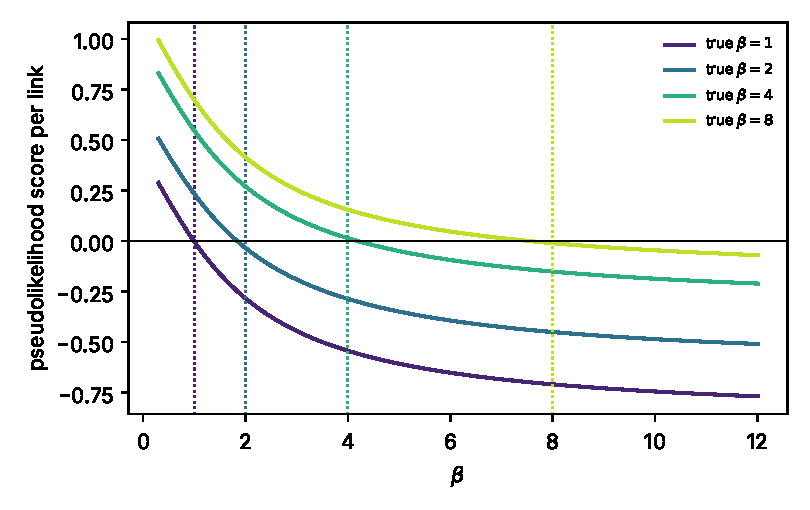
\includegraphics[width=0.85\textwidth]{figures/pl_score.pdf}
\caption[Pseudolikelihood scores for SU(2)]{Pseudolikelihood score per link as a function of $\beta$ for synthetic link conditionals at four true couplings. Each score is decreasing and crosses zero near the true value, marked dotted.}
\label{fig:plscore}
\end{figure}

Figure~\ref{fig:plscore} shows why the equation is easy to solve: the score is monotone and crosses zero steeply. A single configuration of $288$ links fixes the coupling to about fifteen percent at $\beta\le2$ and to about five percent at $\beta\ge4$, with no partition function. The means at $\beta=1$ and $\beta=8$ lie above the true value by about two and a half and four standard errors; we have not diagnosed whether this is a bias of the estimator or of the sampler. Pseudolikelihood is consistent for Gibbs fields under mild conditions, as Comets~\cite{Co92} proved, though not efficient at strong dependence. For the ladder the relevant estimate is not a single $\beta$ but the whole plaquette law, parametrised by its character coefficients $u_n$; the same equations, with the Wilson factor replaced by a character sum, give it.

\subsection{What slicing and Besag give}

Slicing and Besag give three things. The slice variable trick makes the conditionals of heat bath samplers for gauge fields tractable and locates the difficulty in the slice levels, though it does not by itself guarantee fast mixing of the joint chain. In its Riemannian form it would turn the curvature of the group into an explicit log Sobolev constant for the sliced conditional, if the claim above is confirmed, which is a building block for the dynamic route to the gap. And Besag's pseudolikelihood is the right estimator for the empirical renormalization ladder: it fits effective plaquette laws of blocked configurations cheaply, and consistently under mild conditions, which is what testing the Migdal Kadanoff caricature against the real theory requires.

\section*{Exercises}
\begin{enumerate}
\item Prove Kac's lemma for a finite irreducible Markov chain (Section~\ref{sec:c5kaclemma}).
\item Show that the expected number of returns of simple random walk by time $n$ grows like $\log n$ in two dimensions (Section~\ref{sec:c5polya}).
\item Derive the Feynman Kac formula for a bounded continuous potential from the Trotter product formula (Section~\ref{sec:c5fk}).
\item Derive the product estimator and bound its relative variance in terms of the variances of the ratios at each rung (Section~\ref{sec:c5counting}).
\item Write the high temperature expansion of the Ising model and show that its weights are nonnegative for ferromagnetic couplings (Section~\ref{sec:c5positivity}).
\item Write the character expansion of SU(2) lattice gauge theory as a sum over surfaces and identify the analogue of the subgraphs world (Section~\ref{sec:c5positivity}).
\item Show that the variance of a sample mean of a stationary chain is approximately $2\tau_{\mathrm{int}}\sigma^2/n$ (Section~\ref{sec:c5stats}).
\item Derive the Swendsen and Wang conditionals from the Edwards and Sokal joint law, and again by slicing the bond factors as in Higdon's auxiliary variables (Sections~\ref{sec:c5clusters} and~\ref{sec:c5higdon}).
\item Verify the Lee Yang theorem for the Ising model on two sites (Section~\ref{sec:c5zeros}).
\item Show that the slice sampler for a single Cauchy likelihood with a Gaussian prior samples a truncated Gaussian given the slice (Section~\ref{sec:c5slice}).
\item Show that the score of the SU(2) pseudolikelihood has negative derivative in $\beta$ whenever some $k>0$, so that the estimate is unique (Section~\ref{sec:c5pl}).
\item Show that the ICAR precision matrix on a torus has a one dimensional null space (Section~\ref{sec:c5besag}).
\end{enumerate}
